\documentclass{article}
\usepackage{preamble}
\begin{document}
\title{Exploration in \GROOVE}
\author{Arend Rensink}
\date{August 2024}
\maketitle

\section*{Terminology}

\begin{description}
\item[Absence] Equivalent to \emph{absent depth}.

\item[Absent depth (S)] The \emph{absent depth} of a state is the minimal transient depth of that state and all its transitive successors. It follows that the \emph{absent depth} is smaller than or equal to the \emph{transient depth}. As long as a state is not \emph{complete}, its \emph{absent depth} may decrease as a consequence of further exploration.

\item[Absent (S,T)] A state or transition is \emph{absent} if it should not be considered to be part of the state space. In particular, a state is \emph{absent} if it is \emph{complete} and has positive \emph{absent depth}; a transition is \emph{absent} if its target state is \emph{absent}. It follows that an \emph{absent} state is always \emph{transient}. Whether or not a state or transition is \emph{absent} is independent of whether or not it is \emph{inner}.

\item[Atomic (T)] A transition is \emph{atomic} if it is \emph{outer} and consists of a single step, meaning that its source and target states are \emph{steady}.

\item[Closed (S)] A state is \emph{closed} if it is not \emph{open}. A \emph{closed} state may or may not be \emph{complete}.

\item[Complete (S)] A state is \emph{complete} if it is \emph{closed} and all transitive successors up to (but not necessarily including) the first \emph{steady} state are also \emph{closed}. This means that the status of the state is fully known; in particular, it is possible, on the basis of its successors, to decide whether the state is \emph{absent}.

\item[Public (S,T)] A state or transition is \emph{public} if it is both \emph{outer} and \emph{present} (or, in other words, if it is neither \emph{inner} nor \emph{absent}).

\item[Final (S)] A state is \emph{final} if exploration is considered to terminate after reaching it. For instance, if two control blocks are concatenated, the second comes into play after the exploration of the first has reached a final state; also, if a state space is wrapped in an atomic block, the only \emph{steady} states, apart from the \emph{initial} state, are the \emph{final} ones. In other words, \emph{final} has the typical meaning in (regular) automata. A \emph{final} state is certainly \emph{closed} and \emph{steady}; it may or may not have successors.

\item[Initial (S)] A state is \emph{initial} if it is the start state for the exploration. Its \emph{prime} is \emph{steady}.

\item[Incomplete (S)] A state is \emph{incomplete} if it is not \emph{complete}.

\item[Inner (S,T)] A state is \emph{inner} if it is inside the atomic block that makes up the body of a recipe, and a transition is \emph{inner} if it is a step in the execution of a recipe. Hence, an \emph{inner} state is certainly \emph{transient}, but the inverse does not hold. An \emph{inner} state that is not \emph{closed} may still evolve into an \emph{outer} one as a consequence of further exploration.

\item[Open (S)] A state is \emph{open} if its direct outgoing transitions are not fully known. It follows that an open state can become \emph{closed} through further exploration of its outgoing transitions.

\item[Outer (S,T)] A state or transition is \emph{outer} if it is not \emph{inner}.

\item[Partial (T)] A transition is \emph{partial} if it is part of an atomic block. Apart from the \emph{inner} transitions, the \emph{partial} ones include single-step recipe executions.

\item[Present (S,T)] A state or transition is \emph{present} if it is not \emph{absent}. For a state, this means that it either has \emph{absent depth} zero (in which case it will certainly remain \emph{present} under further exploration) or it is \emph{incomplete} (in which case it may become \emph{absent} if, upon becoming \emph{complete}, it has positive \emph{absent depth}).

\item[Prime (S)] The \emph{prime} of a state is the version of that state when it is just discovered, and no outgoing transitions have been explored. Hence, the \emph{prime} is \emph{open}, and may be \emph{transient} even though (because of further exploration) the state itself has become \emph{steady} because its \emph{transient depth} has decreased to zero.

\item[Public (S,T)] A state or transition is \emph{public} if it is both \emph{outer} and \emph{present}.

\item[Steady (S)] A state is \emph{steady} if it is not \emph{transient}.

\item[Transience (S)] Equivalent to \emph{transient depth}.

\item[Transient (S)] A state is \emph{transient} if it is inside an atomic block, meaning that it has a positive \emph{transient depth}. A \emph{transient} state may or may not be \emph{inner}. A transient state that is \emph{open} may still evolve into a \emph{steady} state as a consequence of further exploration.

\item[Transient depth (S)] The \emph{transient depth} of a state is the number of (nested) atomic blocks that it is inside of. A state is \emph{steady} if and only if its \emph{transient depth} is zero; otherwise it is \emph{transient}. As long as a state is not \emph{closed}, its \emph{transient depth} may decrease as a consequence of further exploration.
\end{description}

Figure~\ref{fig:venn} shows these different concepts in relation to each other.

\begin{figure}
\centering
\begin{subfigure}{0.45\textwidth}
\centering
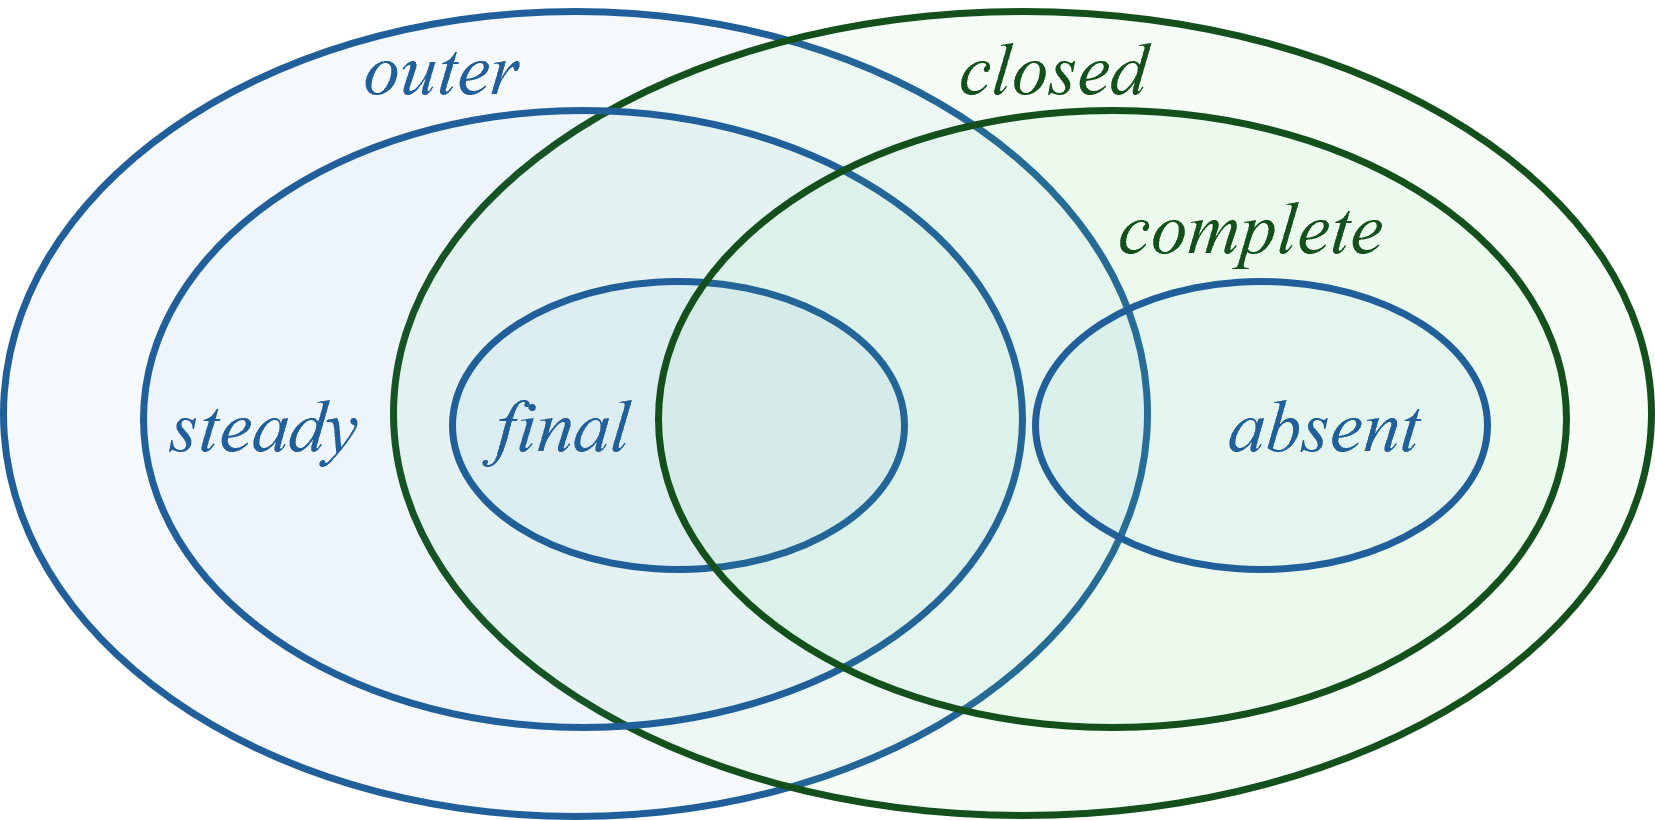
\includegraphics[scale=.4]{figs/s-venn}
\caption{Stats}
\end{subfigure}%
\begin{subfigure}{0.3\textwidth}
\centering
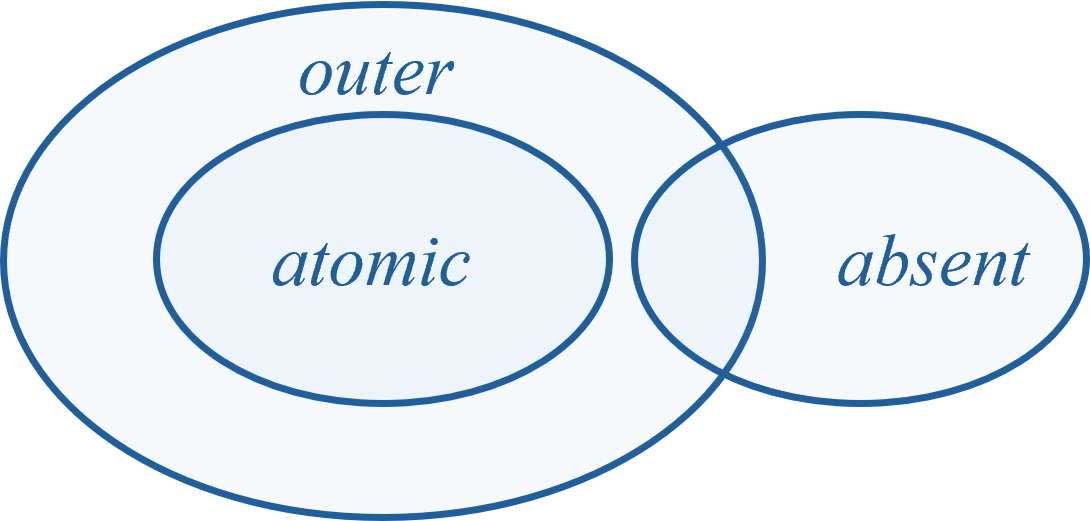
\includegraphics[scale=.4]{figs/t-venn}

\bigskip
\caption{Transitions}
\end{subfigure}%
%
\begin{subfigure}{.25\textwidth}
\scalebox{.8}{$\begin{array}[b]{@{}r@{{\;\equiv\;}}l@{}}
\mathit{inner} & \neg\mathit{outer} \\
\mathit{incomplete} & \neg\mathit{complete} \\
\mathit{open} & \neg\mathit{closed} \\
\mathit{partial} & \neg\mathit{atomic} \\
\mathit{present} & \neg\mathit{absent} \\
\mathit{public} & \mathit{outer} \\
\multicolumn{2}{r}{{}\wedge\mathit{present}} \\
\mathit{transient} & \neg\mathit{steady}
\end{array}$}

\bigskip
\phantomcaption
\end{subfigure}
\caption{Properties of states and transitions}
\label{fig:venn}
\end{figure}


\section*{State spaces}

\medskip\noindent
We globally assume a set of labels $A$.

\medskip\noindent 
A \emph{state space fragment} is a tuple $\cS=\tupof{S,\iota,{\ra},{\up},\TLevel,\Open}$ with
\begin{itemize}
\item $S$ a set of states;
\item $\iota\in S$ the initial state;
\item ${\ra}\subseteq S\times A\times S$ a transition relation;
\item ${\up}\subseteq S$ a termination predicate;
\item ${\TLevel}:S\to \natN$ a \emph{transience level} function;
\item $\Closed\subseteq S$ a set of \emph{closed states}, such that $\up\subseteq \Closed$.
\end{itemize}
%
$\cS$ is called \emph{complete}, or just a \emph{state space}, if $\Closed=S$. A state $s\in S$ is called \emph{final} if $s\up$. We also use a number of auxiliary concepts for states $s\in S$:

\begin{itemize}
\item $\Transient(s)$ expresses that $s$ is \emph{transient}. It is defined by
%
\[ \Transient = \gensetof{s\in S}{\TLevel(s)>0} \enspace. \]

\item $\Steady(s)$ expresses that $s$ is \emph{steady}, which is the inverse of $\Transient(s)$.

\item $\Complete$ expresses that $s$ is \emph{complete}, meaning that $s$ as well as all its $\trans{}$-successors up to and including the first steady state are closed. $\Complete$ is defined as the smallest set such that
%
\[ \Complete = \Closed\cap \bigl(\Steady \cup \gensetof{s\in S}{\forall s\trans{} s'.\, s'\in \Complete\cup \Steady}\bigr) \enspace.
\]
It follows that, if $\cS$ is complete, $\Complete=S$.

\item $\ALevel_C(s)$ is the \emph{absence level} of $s$, meaning the minimum transient depth of $s$ and all its $\trans{}$-successors. It is defined by
%
\[ \ALevel: s\mapsto \min\gensetof{\TLevel(s')}{s\trans{}^* s'} \enspace. \]

\item $\Absent(s)$ expresses that $s$ is \emph{absent}, which is the case if there is no steady state reachable from $s$. It is defined by
%
\[ \Absent= \gensetof{s}{\ALevel(s)>0} \enspace. \]
\end{itemize}

\section*{Pseudo-state spaces}

State spaces are generated from a \emph{pseudo-state spaces}.

\medskip\noindent
A pseudo-state space is a tuple $\cP=\tupof{P,\iota,{\goesto},{\mapsto},{\up},\TLevel,\Recipe}$ with
\begin{itemize}
\item $P$ a finite set of pseudo-states;
\item $\iota\in P$ the initial pseudo-state;
\item ${\goesto}\subseteq P\times P$ a partial order relation called \emph{evolution};
\item ${\step{}}\subseteq P\times A\times P$ a ternary \emph{step relation};
\item ${\up} \subseteq P$ a termination predicate;
\item ${\TLevel}:P\to \natN$ a transience level function;
\item $\Recipe:A\pto A$ a partial \emph{recipe mapping}.
\end{itemize}
A pseudo-state $p\in P$ is called \emph{prime} (denoted $\Prime(p)$) if $p$ is a $\goesto$-minimum, \emph{closed} (denoted $\Closed(p)$) if $p$ is a $\goesto$-maximum and \emph{open} (denoted $\Open(p)$) if it is not closed. $\Transient$ and $\Steady$ are defined using $\TLevel$ as for state space fragments.
%
A pseudo-state space is \emph{well-formed} if it satisfies the following additional properties:
\begin{itemize}
\item Evolution is piecewise linear; i.e., every pseudo-state has at most one direct $\prec$-predecessor and at most one direct $\prec$-successor;
\item Stepping is deterministic; i.e., $\step{}$ is a partial function from $P$ to $A\times P$;
\item All steps go from open to prime pseudo-states; i.e., $p\step{}q$ implies $\Open(p)$ and $\Prime(q)$;
\item All final pseudo-states are steady and closed; i.e., $p\up$ implies $\Steady(p)$ and $\Closed(p)$;
\item Stepping cannot decrease transience; i.e., $p\step{}q$ implies $\TLevel(q)\geq \TLevel(p)$;
\end{itemize}
%
From now on, we only deal with well-formed pseudo-states spaces. The \emph{prime of} and \emph{closure of} a pseudo-state $p$ are defined as
%
\begin{align*}
	\prm p & = q \quad \text{where $\Prime(q)$ and $q\goesto p$} \\
	\cls p & = q \quad \text{where $p\goesto q$ and $\Closed(q)$} \enspace.
\end{align*}
%
Note that these are well-defined because $P$ is finite and $\goesto$ is piecewise linear.

The recipe mapping of a pseudo-state space encodes that an $a$-labelled step for $a\in\dom\Recipe$ kicks off the execution of recipe $\Recipe(a)$ (of which $a$ is the initial partial step). That is, a step $p\step a q$ for which $a\in \dom\Recipe$ gives rise to a $\Recipe(a)$-labelled \emph{recipe transition} in the derived state space, which is considered to be finished upon reaching the first successor $q'$ of $q$ (possibly $q'=q$) for which $\TLevel(q')\leq \TLevel(p)$; unless, that is, $p\step a q$ is itself part of an ongoing recipe transition --- in other words, recipe transitions are not nested. If $a\notin\dom \Recipe$, on the other hand, $p\step a q$ gives rise to an $a$-labelled ``simple'' transition in the derived state space. To capture recipe transitions, we define:
%
\[ p \ttrans{a} \bar q \;\iffdef\; p\step a q_1\leadsto \cdots \leadsto q_n \text{ with } \forall i<n:\TLevel(q_i)>\TLevel(p) \text{ and } \TLevel(q_n)\leq \TLevel(p)
\]
%
in which $\bar q=q_1\cdots q_n$ is a sequence of pseudo-states that the recipe goes through, and $\leadsto$ stands for the union of $\bigcup_{b\in A} \step{b}$ and $\goestostep$ (the direct predecessor relation in $\goesto$).

\medskip\noindent
A pseudo-state space represents a state space in which the states effectively correspond to $\goesto$-ordered sets of pseudo-states (which are actually chains because $\goesto$ is piecewise linear). Rather than formalising the relation in this way, however, we let a state be represented by the initial element of such a chain, i.e., by the (unique) prime pseudo-state.

\medskip\noindent
Given a pseudo-state space $\cP$ as above, a \emph{configuration} is set $C\subseteq P$ of pseudo-states with $\iota\in C$ that is $\goesto$-left-closed (implying, among other things, that $\prm p\in C$ for all $p\in C$) and such that, moreover, $p\in C$ with $p\comesfrom\:\step{} q$ implies $q\in C$. (It follows that $P$ is itself a configuration of $\cP$.) Every configuration $C$ generates a state space $\cS_C= \tupof{S_C,\iota_C,\trans{}_C, \up_C, \TLevel_C}$ as follows:
%
\begin{align*}
S_C & = \gensetof{\prm p}{p\in C} \\
\iota_C & = \iota_\cP \\
{\trans{}_C} & = \gensetof{(\prm p,a,q)}{p,q\in C, a\notin\dom\Recipe, p\step a_\cP q} \\
&\phantom{=} {}\cup \gensetof{(\prm p,\Recipe(a),\prm{q_n})}{p,q_1,\ldots,q_n\in C, a\in\dom\Recipe, p\ttrans a_\cP \bar q} \\
\up_C & = \gensetof{\prm p}{p\in C, p\up_\cP} \\
\TLevel_C & : p \mapsto \min \gensetof{\TLevel_\cP(q)}{p\goesto q\in C} \enspace \text{for all $p\in S_C$} \\
\Closed_C & = \gensetof{\prm p}{p\in C\cap\Closed_\cP} \enspace.
\end{align*}
%
We also use $\Steady_C$, $\Complete_C$, $\ALevel_C$ and $\Absent_C$ to denote $\Steady_{\cS_C}$ etc.

\medskip\noindent
We want to construct $S_P$ incrementally by approaching $P$ through a sequence of configurations, starting with $\setof{\iota}$ and adding, at each iteration, an evolution step $p\goestostep p'$ (denoting that $p'$ is a direct successor of $p$ according to $\goesto$) from $p\in C$ and $p'\notin C$. The latter is defined by 
\[ C\oplus(p,p') = C\cup \setof{p'} \cup \gensetof{q}{p\step a q} \enspace. \]
Incremental construction means that, if $D=C\oplus(p,p')$, all components of $S_D$ can be constructed from $S_C$ and $\cP$. Indeed, we have
%
\begin{align*}
\up_D & = \up_C \cup \gensetof{\prm{p'}}{p'\up_\cP} \\
\TLevel_D & : s\mapsto
  \begin{cases}
  \TLevel_\cP(p') & \text{if $s=\prm{p'}$} \\
  \TLevel_\cP(q) & \text{if $s=q\notin S_C$} \\
  \TLevel_C(s) & \text{otherwise}
  \end{cases} \\
\Closed_D & = \Closed_C \cup\gensetof{\prm{p'}}{p'\in \Closed_\cP} \\
\Steady_D & = \Steady_C \cup \gensetof{\prm{p'}}{p'\in\Steady_\cP} \enspace.
\end{align*}
%
The incremental construction of $\Complete_C$, $\ALevel_C$ and especially $\trans{}_C$, however, is less straightforward, because all of those involve paths of unbounded length. In particular, the inclusion (or ``exploration'') of a new step $p\step a q$ of the pseudo-state space into a configuration may generate recipe transitions that start in a predecessor of $p$ and end in a successor of $q$. For the purpose of this construction, we therefore introduce several auxiliary data structures.

\begin{itemize}
\item A transition $t\trans{a}_C t$ is \emph{partial} if it starts in a $\cP$-transient state:
%
\[ \Partial_C = \gensetof{(s,a,t)\in {\trans{}_C}}{\Transient(s)} \]

\item 
%
\[ \RS_C : s \mapsto \gensetof{(t,a,t')\in \Partial_C}{\Transient(t), s\trans{}_C^* t\trans a_C t'} \]

\item For a given state $s$, the \emph{reachable transient open states} are the $C$-open states reachable through a (possibly empty) sequence of $\trans{}_C$-transitions between $\cP$-transient states.
%
\[ \RTO_C : s \mapsto \gensetof{t\in S_C\setminus \Closed_C}{s\trans{}_C^* t} \]

\end{itemize}
\end{document}
